\documentclass[../DoAn.tex]{subfiles}
\usepackage{indentfirst}
\begin{document}

\section{Đặt vấn đề}
\label{section:1.1}
Hiện nay, sự phát triển và bùng nổ dữ liệu lớn là một trong những xu hướng chủ yếu trong thế giới công nghiệp. Dữ liệu đang tăng nhanh chóng và dự báo sẽ tiếp tục tăng trong tương lai. Các nguồn dữ liệu khác nhau như IoT (Internet of Things), máy tính, máy tính xách tay, mạng xã hội, cửa hàng bán lẻ, trực tuyến, các nền tảng livestream v..v đang tạo ra lượng dữ liệu lớn mỗi ngày với những con số ấn tượng như trong mỗi phút 4.7 triệu video được xem trên Youtube, 1.400 lượt tải xuống trên nền tảng Tiktok, 19 triệu tin nhắn được gửi đi, 1.3 triệu lượt đăng nhập tài khoản Facebook,.. Theo IDC tổng dung lượng dữ liệu trên toàn thế giới đến năm 2025 có thể đạt lên đến 175 Zettabytes (175 tỉ Terabytes). Với việc bùng nổ của dữ liệu (kích thước, định dạng, tốc độ sinh) đã dẫn đến nhu cầu giải quyết bài toán tích hợp dữ liệu nhằm kết hợp dữ liệu từ nhiều nguồn về một định dạng chung thống nhất giúp việc quản lý, phân tích, khai thác dữ liệu lớn hiệu quả hỗ trợ việc ra quyết định tăng khả năng cạnh tranh cũng như doanh thu của doanh nghiệp. Ứng dụng của tích hợp dữ liệu trên thực tế đang được ứng dụng vào rất nhiều lĩnh vục của đời sống như kinh doanh, khoa học, bán lẻ,.. 

% 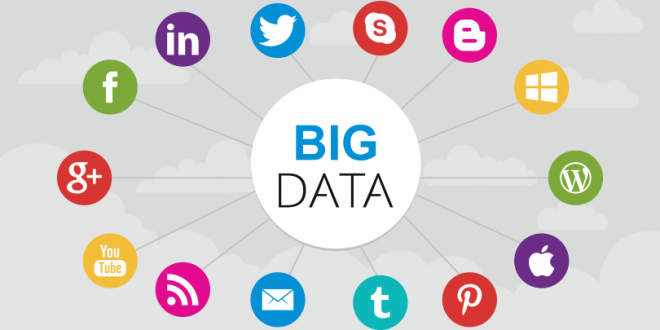
\includegraphics[scale=0.8]{Hinhve/bigdata.png}
\begin{figure}[H]
    \centering
    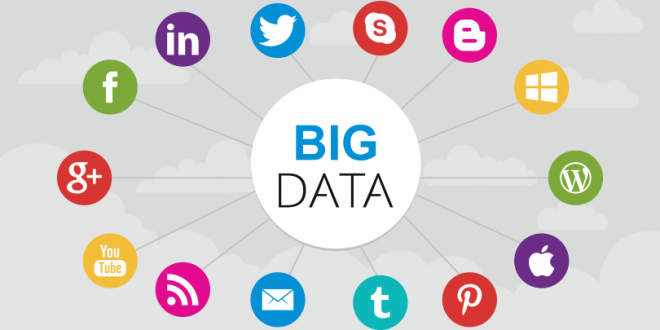
\includegraphics[scale=0.9]{Hinhve/bigdata.png}
    \caption{Bùng nổ dữ liệu lớn - BigData}
    \label{fig:my_label2}
\end{figure}

Tích hợp dữ liệu đóng vai trò quan trọng trong các hoạt động kinh doanh bằng việc cung cấp một tập dữ liệu thống nhất tích hợp từ nhiều nguồn cho phép doanh nghiệp đưa ra chiến lược, quyết định kinh doanh hợp lý. Một vài ứng dụng chính của tích hợp dữ liệu trong kinh doanh như giúp cho hệ thống hoạt động hiệu quả hơn nhờ vào việc tự động các quy trình và giảm thiểu các bước lưu trữ dự liệu trung gian thủ công hay tích hợp dữ liệu khách hàng từ các nguồn khác nhau cung cấp một cái nhìn tổng quan đầy đủ về dữ liệu tăng trải nghiệm, hài lòng người dùng. Bên cạnh đó tích hợp dữ liệu giúp doanh nghiệp xác định và giảm thiểu những rủi ro bằng việc cung cấp bức tranh toàn cảnh, hoàn chỉnh về các yếu tố rủi ro và xu hướng của chúng. Ngày nay tích hợp dữ liệu được ứng dụng trong kinh doanh để hỗ trợ việc ra quyết định chiến lược, giúp hệ thống vận hành hiệu quả  hơn và tăng khả năng cạnh tranh trên thị trường.

Trong nghiên cứu khoa học tích hợp dữ liệu giúp kết nối các nguồn dữ liệu khác nhau dể tạo ra một cái nhìn tổng thể toàn diện hơn về một chủ đề hoặc vấn đề nghiên cứu đồng thời giúp quản lý dữ liệu từ các nguồn tránh trùng lặp dữ liệu bằng việc sử dụng công nghệ lưu trữ xử lý dữ liệu lớn như big data và điện toán đám mây. Ngoài ra một vài ứng dụng khác trong khoa học điển hình như hỗ trợ xây dựng mô hình học máy, mô hình thống kê sử dụng kĩ thuật machine learning và deep learning hay được sử dụng để đánh giá mức độ hiệu quả chiến lược hoặc giải pháp  trong các lĩnh vực chăm sóc sức khỏe, tài chính và kinh doanh.

Tích hợp dữ liệu đặc biệt quan trọng trong ngành chăm sóc sức khỏe. Dữ liệu tích hợp từ hồ sơ bệnh nhân của các phòng khám khác nhau giúp bác sĩ lâm sàng xác định bệnh và rối loạn y tế bằng cách tích hợp dữ liệu từ nhiều hệ thống bệnh viện, phòng khám khác nhau vào một góc nhìn thông tin hữu ích nhất để suy luận chuẩn đoán những thông tin có độ chính xác cao. Việc thu thập và tích hợp dữ liệu hiệu quả cũng cải thiện độ chính xác của quá trình xử lý yêu cầu bảo hiểm y tế và đảm bảo rằng tên bệnh nhân và thông tin liên hệ được ghi lại một cách nhất quán và chính xác. Khả năng tương tác đề cập đến việc chia sẻ thông tin trên các hệ thống khác nhau.

Tích hợp dữ liệu web cũng đang là chủ đề được quan tâm trong những năm gần đây cùng với sự bùng nổ của dữ liệu lớn trong đó dữ liệu các trang web trên Internet ở khắp mọi nơi. Có hàng triệu các bảng biểu chất lượng cao trên Internet, hay đến việc tạo một web site được tích hợp dữ liệu từ rất nhiều trang web khác nhau phục vụ các bài toán so sánh giá các sản phẩm thương mại điện từ hay thông tin về việc làm tuyển dụng giúp cho việc tra cứu một cách dễ dàng chỉ bằng thao tác click vào tên của nó.

\section{Mục tiêu và phạm vi đề tài}
\label{section:1.2}
Ngày nay, điện thoại thông minh trở nên phổ biến rộng rãi đối với tất cả mọi người mọi hoàn cảnh. Nhu cầu mua sắm điện thoại ngày càng cao kéo theo sự phát triển ra đời của các cửa hàng, trung tâm, hãng sản xuất để phục vụ đáp ứng cho người dùng. Tuy nhiên điều này cũng gây khó khăn cho người tiêu dùng khi muốn mua lựa chọn một sản phẩm phù hợp với chính mình về giá cả, về chất lượng, nhà cung cấp ,… Đứng trước tình hình đó trong học phần đồ án tốt nghiệp này em quyết định xây dựng một hệ thống tích hợp dữ liệu từ các trang web cửa hàng bán điện thoại cho phép người dùng có thể so sánh giá mà cụ thể hơn là giá của sản phẩm đến từ Apple (điện thoại, ipad, macbook, applewatch,..) Nhờ đó người dùng có nhiều lựa chọn và cái nhìn tổng quan hơn về sản phẩm, bên cạnh đó hiển thị chi tiết thông số kĩ thuật của sản phẩm và một số phân tích biểu đồ trực quan của thị trường sản phẩm Apple.

\section{Định hướng giải pháp}
\label{section:1.3}
Xác định được bài toán tích hợp dữ liệu các sản phẩm Apple em đề xuất định hướng giải pháp xây dựng hệ thống tích hợp dữ liệu từ nhiều nguồn theo cách tiếp cận kho dữ liệu (data warehouse). Cụ thể hệ thống sẽ có pha thu thập dữ liệu từ các nguồn khác nhau là các hệ thống bán điện thoại uy tín (cellphoneS, thegioididong, viettelstore,…) Dữ liệu sau khi được thu thập sẽ được làm sạch tiền xử lý theo đúng định dạng và làm đầu vào cho pha tích hợp dữ liệu về một tập dữ liệu thống nhất. Mục đích cuối cùng của pha này là tạo ra một tạp dữ liệu tích hợp từ các nguồn trên phục vụ cho hệ thống tìm kiếm và luôn trong trạng thái sẵn sàng. Vì vậy hệ thống cơ sở dữ liệu phải có tính chịu lỗi cao nên em lựa chọn cơ sở dữ liệu MongoDB Cloud là một cơ sở dữ liệu dạng NoSQL có thể lưu trữ dữ liệu linh hoạt hơn. Sau khi đồng bộ dữ liệu lên đám mây, dữ liệu sẽ được truy xuất từ hệ thống tìm kiếm cho phép người dùng so sánh giá của các sản phẩm Apple, thông số kĩ thuật và một vài phân tích liên quan.

\section{Bố cục đồ án}
\label{section:1.4}
Phần còn lại của báo cáo đồ án tốt nghiệp này được tổ chức như sau 

Chương 2 trình bày về khảo sát và phân tích yêu cầu. Nội dung chính của chương này nhằm khảo sát chi tiết về hiện trạng và yêu cầu của phần mềm. Và cuối cùng là tổng quan về các chức năng cơ bản ứng dụng của hệ thống.

Chương 3 trình bày về các công nghệ được sử dụng trong hệ thống để giải quyết được bài toán. Nọi dung của chương được chia thành các hệ thống khác nhau: hệ thống thu thập dữ liệu (Selenium, Scrapy), hệ thống lưu trữ và xử lý dữ liệu (Kafka, MongoDB) và hệ thống web tìm kiếm (Springboot, ReactJs) 

Chương 4 Xây dựng hệ thống tích hợp dữ liệu trình bày đóng góp chính của đồ án. Đó là một hệ thống hoàn chỉnh từ pha thu thập dữ liệu tiền xử lý lưu trữ dữ liệu đến pha ứng dụng cho phép người dùng thao tác và tìm kiếm dữ liệu đã được xử lý.

Chương 5 kết luận và hướng phát triển để mở rộng quy mô cũng như tính chất của bài toán tích hợp dữ liệu
\end{document}